%%%%%%%%%%%%%%%%%%%%%%%%%%%%%%%%%%%%%%%%%%%%%%%%%%%%%%%%%%%%%%%%%%%%%%%%%%%%%%%%
% CHAPTER 4
%%%%%%%%%%%%%%%%%%%%%%%%%%%%%%%%%%%%%%%%%%%%%%%%%%%%%%%%%%%%%%%%%%%%%%%%%%%%%%%%

\chapter{Fourier Series}

\begin{tcolorbox}[colback=blue!5!white,colframe=blue!70!black,title=Learning Objectives]

After studying this chapter, the reader will be able to

\begin{itemize}
\item Understand the idea of representing periodic signals as sums of sinusoids.
\item Write the trigonometric Fourier series representation.
\item Derive the Fourier coefficients.
\item Use orthogonality of sine and cosine functions.
\item Determine coefficients for even and odd signals.
\item Find the Fourier series of common waveforms.
\end{itemize}

\end{tcolorbox}

%%%%%%%%%%%%%%%%%%%%%%%%%%%%%%%%%%%%%%%%%%%%%%%%%%%%%%%%%%%%%%%%%%%%%%%%%%%%%%%%

\section{Introduction}

Any periodic signal can be represented as a sum of sinusoidal signals of
different frequencies, amplitudes and phases.

This representation is called the \textbf{Fourier Series}.

The fundamental idea is

\[
\boxed{
\text{Periodic signal}
=
\text{DC component}
+
\text{Harmonics}
}
\]

where the harmonics are sinusoidal components whose frequencies are integer
multiples of the fundamental frequency.

Fourier Series forms the foundation of

\begin{itemize}
\item communication systems,
\item modulation,
\item spectrum analysis,
\item filter design,
\item and digital signal processing.
\end{itemize}

%%%%%%%%%%%%%%%%%%%%%%%%%%%%%%%%%%%%%%%%%%%%%%%%%%%%%%%%%%%%%%%%%%%%%%%%%%%%%%%%

\section{Periodic Signal}

A signal is periodic if

\[
\boxed{
x(t)=x(t+T)
}
\]

where \(T\) is the fundamental period.

The fundamental frequency is

\[
\boxed{
f_0=\frac{1}{T}
}
\]

and the fundamental angular frequency is

\[
\boxed{
\omega_0=\frac{2\pi}{T}
}
\]

%%%%%%%%%%%%%%%%%%%%%%%%%%%%%%%%%%%%%%%%%%%%%%%%%%%%%%%%%%%%%%%%%%%%%%%%%%%%%%%%

\section{Harmonics}

The frequencies present in a Fourier series are

\[
f_0,\ 2f_0,\ 3f_0,\ldots,nf_0.
\]

The \(n\)-th harmonic has angular frequency

\[
\boxed{
n\omega_0
}
\]

%%%%%%%%%%%%%%%%%%%%%%%%%%%%%%%%%%%%%%%%%%%%%%%%%%%%%%%%%%%%%%%%%%%%%%%%%%%%%%%%

\section{Trigonometric Fourier Series}

A periodic signal \(x(t)\) with period \(T\) can be written as

\[
\boxed{
x(t)=
\frac{a_0}{2}
+
\sum_{n=1}^{\infty}
\left[
a_n\cos(n\omega_0 t)
+
b_n\sin(n\omega_0 t)
\right]
}
\]

where

\begin{itemize}
\item \(a_0\): DC coefficient,
\item \(a_n\): cosine coefficients,
\item \(b_n\): sine coefficients.
\end{itemize}

%%%%%%%%%%%%%%%%%%%%%%%%%%%%%%%%%%%%%%%%%%%%%%%%%%%%%%%%%%%%%%%%%%%%%%%%%%%%%%%%

\section{Orthogonality of Trigonometric Functions}

%%%%%%%%%%%%%%%%%%%%%%%%%%%%%%%%%%%%%%%%%%%%%%%%%%%%%%%%%%%%%%%%%%%%%%%%%%%%%%%%

\subsection{Cosine Functions}

\[
\int_0^T
\cos(m\omega_0 t)\cos(n\omega_0 t)\,dt
=
\begin{cases}
0, & m\neq n\\[4pt]
\dfrac{T}{2}, & m=n
\end{cases}
\]

%%%%%%%%%%%%%%%%%%%%%%%%%%%%%%%%%%%%%%%%%%%%%%%%%%%%%%%%%%%%%%%%%%%%%%%%%%%%%%%%

\subsection{Sine Functions}

\[
\int_0^T
\sin(m\omega_0 t)\sin(n\omega_0 t)\,dt
=
\begin{cases}
0, & m\neq n\\[4pt]
\dfrac{T}{2}, & m=n
\end{cases}
\]

%%%%%%%%%%%%%%%%%%%%%%%%%%%%%%%%%%%%%%%%%%%%%%%%%%%%%%%%%%%%%%%%%%%%%%%%%%%%%%%%

\subsection{Sine and Cosine}

\[
\boxed{
\int_0^T
\sin(m\omega_0 t)\cos(n\omega_0 t)\,dt=0
}
\]

These orthogonality relations allow us to extract individual Fourier
coefficients.

%%%%%%%%%%%%%%%%%%%%%%%%%%%%%%%%%%%%%%%%%%%%%%%%%%%%%%%%%%%%%%%%%%%%%%%%%%%%%%%%

\section{Derivation of \(a_0\)}

Multiply the Fourier series by 1 and integrate over one period:

\[
\int_0^T x(t)\,dt
=
\int_0^T
\left[
\frac{a_0}{2}
+\sum_{n=1}^{\infty}(\cdots)
\right]dt
\]

All sine and cosine integrals become zero over one complete period, leaving

\[
\int_0^T x(t)\,dt
=
\frac{a_0}{2}T
\]

Hence,

\[
\boxed{
a_0=\frac{2}{T}\int_0^T x(t)\,dt
}
\]

%%%%%%%%%%%%%%%%%%%%%%%%%%%%%%%%%%%%%%%%%%%%%%%%%%%%%%%%%%%%%%%%%%%%%%%%%%%%%%%%

\section{Derivation of \(a_n\)}

Multiply the Fourier series by \(\cos(m\omega_0 t)\) and integrate:

\[
\int_0^T x(t)\cos(m\omega_0 t)\,dt
=
\frac{a_mT}{2}
\]

Therefore,

\[
\boxed{
a_n=
\frac{2}{T}
\int_0^T
x(t)\cos(n\omega_0 t)\,dt
}
\]

%%%%%%%%%%%%%%%%%%%%%%%%%%%%%%%%%%%%%%%%%%%%%%%%%%%%%%%%%%%%%%%%%%%%%%%%%%%%%%%%

\section{Derivation of \(b_n\)}

Multiply the Fourier series by \(\sin(m\omega_0 t)\) and integrate:

\[
\int_0^T x(t)\sin(m\omega_0 t)\,dt
=
\frac{b_mT}{2}
\]

Hence,

\[
\boxed{
b_n=
\frac{2}{T}
\int_0^T
x(t)\sin(n\omega_0 t)\,dt
}
\]

%%%%%%%%%%%%%%%%%%%%%%%%%%%%%%%%%%%%%%%%%%%%%%%%%%%%%%%%%%%%%%%%%%%%%%%%%%%%%%%%

\section{Summary of Fourier Coefficients}

\begin{tcolorbox}[title=Coefficient Formulas,colback=yellow!10]

\[
a_0=
\frac{2}{T}\int_0^T x(t)\,dt
\]

\[
a_n=
\frac{2}{T}
\int_0^T x(t)\cos(n\omega_0 t)\,dt
\]

\[
b_n=
\frac{2}{T}
\int_0^T x(t)\sin(n\omega_0 t)\,dt
\]

\end{tcolorbox}

%%%%%%%%%%%%%%%%%%%%%%%%%%%%%%%%%%%%%%%%%%%%%%%%%%%%%%%%%%%%%%%%%%%%%%%%%%%%%%%%

\section{Even and Odd Signals}

%%%%%%%%%%%%%%%%%%%%%%%%%%%%%%%%%%%%%%%%%%%%%%%%%%%%%%%%%%%%%%%%%%%%%%%%%%%%%%%%

\subsection{Even Signal}

If

\[
x(t)=x(-t),
\]

then

\[
\boxed{
b_n=0
}
\]

Only cosine terms remain:

\[
x(t)=
\frac{a_0}{2}
+
\sum_{n=1}^{\infty}
a_n\cos(n\omega_0 t)
\]

The coefficients can be computed as

\[
\boxed{
a_n=
\frac{4}{T}
\int_0^{T/2}
x(t)\cos(n\omega_0 t)\,dt
}
\]

%%%%%%%%%%%%%%%%%%%%%%%%%%%%%%%%%%%%%%%%%%%%%%%%%%%%%%%%%%%%%%%%%%%%%%%%%%%%%%%%

\section{Odd Signal}

If

\[
x(t)=-x(-t),
\]

then

\[
\boxed{
a_0=0,\qquad a_n=0
}
\]

Only sine terms remain:

\[
x(t)=
\sum_{n=1}^{\infty}
b_n\sin(n\omega_0 t)
\]

and

\[
\boxed{
b_n=
\frac{4}{T}
\int_0^{T/2}
x(t)\sin(n\omega_0 t)\,dt
}
\]

%%%%%%%%%%%%%%%%%%%%%%%%%%%%%%%%%%%%%%%%%%%%%%%%%%%%%%%%%%%%%%%%%%%%%%%%%%%%%%%%

\section{Half-Wave Symmetry}

A signal has half-wave symmetry if

\[
\boxed{
x\left(t+\frac{T}{2}\right)=-x(t)
}
\]

For such signals,

\[
\boxed{
a_0=0
}
\]

and all even harmonics vanish:

\[
\boxed{
a_{2k}=0,\qquad b_{2k}=0
}
\]

Only odd harmonics are present.

%%%%%%%%%%%%%%%%%%%%%%%%%%%%%%%%%%%%%%%%%%%%%%%%%%%%%%%%%%%%%%%%%%%%%%%%%%%%%%%%

\section{Example: Pure Cosine}

Let

\[
x(t)=A\cos(\omega_0 t).
\]

Comparing with the Fourier series,

\[
a_1=A,
\qquad
a_n=0\ (n\neq1),
\qquad
b_n=0,
\qquad
a_0=0.
\]

Thus, a single sinusoid contains only one harmonic component.

%%%%%%%%%%%%%%%%%%%%%%%%%%%%%%%%%%%%%%%%%%%%%%%%%%%%%%%%%%%%%%%%%%%%%%%%%%%%%%%%

\section{Example: DC Signal}

Let

\[
x(t)=A.
\]

Then

\[
a_0=
\frac{2}{T}\int_0^T A\,dt
=
2A.
\]

Therefore,

\[
\frac{a_0}{2}=A
\]

and all other coefficients are zero.

%%%%%%%%%%%%%%%%%%%%%%%%%%%%%%%%%%%%%%%%%%%%%%%%%%%%%%%%%%%%%%%%%%%%%%%%%%%%%%%%

\section{Graphical Interpretation}

The Fourier series decomposes a periodic waveform into

\begin{itemize}
\item a constant (DC) component,
\item a fundamental sinusoid,
\item and higher-order harmonics.
\end{itemize}

\begin{center}
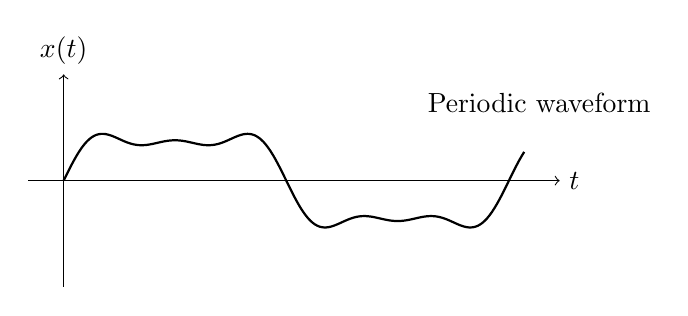
\begin{tikzpicture}[scale=0.9]
\draw[->] (-0.5,0) -- (7,0) node[right] {$t$};
\draw[->] (0,-1.5) -- (0,1.5) node[above] {$x(t)$};

\draw[thick,smooth,samples=100,domain=0:6.5]
plot(\x,{0.7*sin(deg(\x))+0.25*sin(deg(3*\x))+0.12*sin(deg(5*\x))});

\node[right] at (5,1.1) {Periodic waveform};
\end{tikzpicture}
\end{center}

This waveform can be viewed as the sum of the fundamental, third harmonic and
fifth harmonic.

%%%%%%%%%%%%%%%%%%%%%%%%%%%%%%%%%%%%%%%%%%%%%%%%%%%%%%%%%%%%%%%%%%%%%%%%%%%%%%%%

\section{Why Fourier Series Works}

Sinusoids form an orthogonal basis over one period. Just as any vector can be
expressed as a combination of orthogonal unit vectors, any periodic signal can
be expressed as a combination of orthogonal sine and cosine functions.

%%%%%%%%%%%%%%%%%%%%%%%%%%%%%%%%%%%%%%%%%%%%%%%%%%%%%%%%%%%%%%%%%%%%%%%%%%%%%%%%

\begin{tcolorbox}[title=Quick Recall,colback=blue!5]

\[
\omega_0=\frac{2\pi}{T}
\]

\[
x(t)=
\frac{a_0}{2}
+\sum_{n=1}^{\infty}
\left[
a_n\cos(n\omega_0 t)+b_n\sin(n\omega_0 t)
\right]
\]

\[
a_0=
\frac{2}{T}\int_0^T x(t)\,dt
\]

\[
a_n=
\frac{2}{T}\int_0^T x(t)\cos(n\omega_0 t)\,dt
\]

\[
b_n=
\frac{2}{T}\int_0^T x(t)\sin(n\omega_0 t)\,dt
\]

Even signal \(\Rightarrow b_n=0\)

Odd signal \(\Rightarrow a_0=a_n=0\)

Half-wave symmetry \(\Rightarrow\) only odd harmonics

\end{tcolorbox}
%%%%%%%%%%%%%%%%%%%%%%%%%%%%%%%%%%%%%%%%%%%%%%%%%%%%%%%%%%%%%%%%%%%%%%%%%%%%%%%%
%%%%%%%%%%%%%%%%%%%%%%%%%%%%%%%%%%%%%%%%%%%%%%%%%%%%%%%%%%%%%%%%%%%%%%%%%%%%%%%%
\section{Exponential Fourier Series}

%%%%%%%%%%%%%%%%%%%%%%%%%%%%%%%%%%%%%%%%%%%%%%%%%%%%%%%%%%%%%%%%%%%%%%%%%%%%%%%%

\subsection{Euler's Formula}

Using

\[
e^{j\theta}=\cos\theta+j\sin\theta,
\]

the trigonometric Fourier series can be written in a compact exponential form.

%%%%%%%%%%%%%%%%%%%%%%%%%%%%%%%%%%%%%%%%%%%%%%%%%%%%%%%%%%%%%%%%%%%%%%%%%%%%%%%%

\subsection{Exponential Form}

\[
\boxed{
x(t)=\sum_{n=-\infty}^{\infty}C_n e^{jn\omega_0 t}
}
\]

where \(C_n\) are the complex Fourier coefficients.

%%%%%%%%%%%%%%%%%%%%%%%%%%%%%%%%%%%%%%%%%%%%%%%%%%%%%%%%%%%%%%%%%%%%%%%%%%%%%%%%

\section{Derivation of \(C_n\)}

Multiply both sides by \(e^{-jm\omega_0 t}\) and integrate over one period:

\[
\int_0^T x(t)e^{-jm\omega_0 t}dt
=
\sum_{n=-\infty}^{\infty}
C_n
\int_0^T
e^{j(n-m)\omega_0 t}dt
\]

Using orthogonality,

\[
\int_0^T e^{j(n-m)\omega_0 t}dt=
\begin{cases}
T, & n=m\\
0, & n\neq m
\end{cases}
\]

Therefore,

\[
\boxed{
C_n=
\frac{1}{T}
\int_0^T
x(t)e^{-jn\omega_0 t}dt
}
\]

%%%%%%%%%%%%%%%%%%%%%%%%%%%%%%%%%%%%%%%%%%%%%%%%%%%%%%%%%%%%%%%%%%%%%%%%%%%%%%%%

\section{Relationship Between \(C_n\) and \(a_n,b_n\)}

\[
\boxed{
C_0=\frac{a_0}{2}
}
\]

For \(n>0\),

\[
\boxed{
C_n=\frac{1}{2}(a_n-jb_n)
}
\]

\[
\boxed{
C_{-n}=\frac{1}{2}(a_n+jb_n)
}
\]

%%%%%%%%%%%%%%%%%%%%%%%%%%%%%%%%%%%%%%%%%%%%%%%%%%%%%%%%%%%%%%%%%%%%%%%%%%%%%%%%

\section{Magnitude and Phase Spectrum}

The coefficient \(C_n\) is complex:

\[
C_n=|C_n|e^{j\angle C_n}.
\]

Thus,

\begin{itemize}
\item \(|C_n|\): magnitude spectrum,
\item \(\angle C_n\): phase spectrum.
\end{itemize}

%%%%%%%%%%%%%%%%%%%%%%%%%%%%%%%%%%%%%%%%%%%%%%%%%%%%%%%%%%%%%%%%%%%%%%%%%%%%%%%%

\subsection{Line Spectrum}

For periodic signals, the spectrum consists of discrete lines at

\[
\omega=n\omega_0.
\]

\begin{center}
\begin{tikzpicture}[scale=0.9]
\draw[->] (-4,0) -- (4,0) node[right] {$\omega$};
\draw[->] (0,0) -- (0,3) node[above] {$|C_n|$};

\foreach \x/\h in {-3/0.8,-2/1.4,-1/2.2,1/2.2,2/1.4,3/0.8}{
  \draw[thick] (\x,0) -- (\x,\h);
}
\end{tikzpicture}
\end{center}

This is called a \textbf{line spectrum}.

%%%%%%%%%%%%%%%%%%%%%%%%%%%%%%%%%%%%%%%%%%%%%%%%%%%%%%%%%%%%%%%%%%%%%%%%%%%%%%%%

\section{Parseval's Theorem}

The average power of a periodic signal is

\[
P=
\frac{1}{T}\int_0^T |x(t)|^2dt.
\]

Using Fourier coefficients,

\[
\boxed{
P=
\sum_{n=-\infty}^{\infty}|C_n|^2
}
\]

In trigonometric form,

\[
\boxed{
P=
\frac{a_0^2}{4}
+
\frac{1}{2}
\sum_{n=1}^{\infty}(a_n^2+b_n^2)
}
\]

Parseval's theorem relates time-domain power to frequency-domain power.

%%%%%%%%%%%%%%%%%%%%%%%%%%%%%%%%%%%%%%%%%%%%%%%%%%%%%%%%%%%%%%%%%%%%%%%%%%%%%%%%

\section{Square Wave}

Consider the odd square wave

\[
x(t)=
\begin{cases}
A, & 0<t<T/2\\
-A, & -T/2<t<0
\end{cases}
\]

This signal is odd, so

\[
a_0=0,\qquad a_n=0.
\]

%%%%%%%%%%%%%%%%%%%%%%%%%%%%%%%%%%%%%%%%%%%%%%%%%%%%%%%%%%%%%%%%%%%%%%%%%%%%%%%%

\subsection{Compute \(b_n\)}

\[
b_n=
\frac{4}{T}
\int_0^{T/2}
A\sin(n\omega_0 t)\,dt
\]

\[
=
\frac{4A}{T}
\left[
-\frac{\cos(n\omega_0 t)}{n\omega_0}
\right]_0^{T/2}
\]

Since

\[
\omega_0=\frac{2\pi}{T},
\qquad
\cos(n\pi)=(-1)^n,
\]

we get

\[
\boxed{
b_n=
\frac{2A}{n\pi}
\left(1-(-1)^n\right)
}
\]

Thus,

\[
b_n=
\begin{cases}
\dfrac{4A}{n\pi}, & n\ \text{odd}\\[6pt]
0, & n\ \text{even}
\end{cases}
\]

%%%%%%%%%%%%%%%%%%%%%%%%%%%%%%%%%%%%%%%%%%%%%%%%%%%%%%%%%%%%%%%%%%%%%%%%%%%%%%%%

\subsection{Final Fourier Series}

\[
\boxed{
x(t)=
\frac{4A}{\pi}
\left[
\sin\omega_0 t
+\frac{1}{3}\sin3\omega_0 t
+\frac{1}{5}\sin5\omega_0 t
+\cdots
\right]
}
\]

Only odd harmonics are present.

%%%%%%%%%%%%%%%%%%%%%%%%%%%%%%%%%%%%%%%%%%%%%%%%%%%%%%%%%%%%%%%%%%%%%%%%%%%%%%%%

\section{Rectangular Pulse Train}

Consider

\[
x(t)=
\begin{cases}
A, & |t|<\tau/2\\
0, & \tau/2<|t|<T/2
\end{cases}
\]

This signal is even, so \(b_n=0\).

%%%%%%%%%%%%%%%%%%%%%%%%%%%%%%%%%%%%%%%%%%%%%%%%%%%%%%%%%%%%%%%%%%%%%%%%%%%%%%%%

\subsection{DC Component}

\[
a_0=
\frac{4}{T}
\int_0^{\tau/2}A\,dt
=
\frac{2A\tau}{T}
\]

%%%%%%%%%%%%%%%%%%%%%%%%%%%%%%%%%%%%%%%%%%%%%%%%%%%%%%%%%%%%%%%%%%%%%%%%%%%%%%%%

\subsection{Cosine Coefficients}

\[
a_n=
\frac{4A}{T}
\int_0^{\tau/2}
\cos(n\omega_0 t)\,dt
\]

\[
=
\frac{4A}{T}
\frac{\sin(n\omega_0\tau/2)}{n\omega_0}
\]

Using \(\omega_0=2\pi/T\),

\[
\boxed{
a_n=
\frac{2A}{n\pi}
\sin\left(\frac{n\pi\tau}{T}\right)
}
\]

%%%%%%%%%%%%%%%%%%%%%%%%%%%%%%%%%%%%%%%%%%%%%%%%%%%%%%%%%%%%%%%%%%%%%%%%%%%%%%%%

\subsection{Duty Cycle}

Define

\[
\boxed{
D=\frac{\tau}{T}
}
\]

Then,

\[
\boxed{
a_n=
\frac{2A}{n\pi}\sin(n\pi D)
}
\]

This is one of the most important Fourier-series results.

%%%%%%%%%%%%%%%%%%%%%%%%%%%%%%%%%%%%%%%%%%%%%%%%%%%%%%%%%%%%%%%%%%%%%%%%%%%%%%%%

\section{Sawtooth Wave}

Consider

\[
x(t)=\frac{2A}{T}t,
\qquad
-\frac{T}{2}<t<\frac{T}{2}.
\]

This signal is odd, so only sine terms exist.

%%%%%%%%%%%%%%%%%%%%%%%%%%%%%%%%%%%%%%%%%%%%%%%%%%%%%%%%%%%%%%%%%%%%%%%%%%%%%%%%

\subsection{Coefficient}

\[
b_n=
\frac{4}{T}
\int_0^{T/2}
\frac{2A}{T}t\sin(n\omega_0 t)\,dt
\]

Using integration by parts,

\[
\boxed{
b_n=
\frac{2A}{n\pi}(-1)^{n+1}
}
\]

%%%%%%%%%%%%%%%%%%%%%%%%%%%%%%%%%%%%%%%%%%%%%%%%%%%%%%%%%%%%%%%%%%%%%%%%%%%%%%%%

\subsection{Final Series}

\[
\boxed{
x(t)=
\frac{2A}{\pi}
\left[
\sin\omega_0 t
-\frac{1}{2}\sin2\omega_0 t
+\frac{1}{3}\sin3\omega_0 t
-\cdots
\right]
}
\]

Both even and odd harmonics are present.

%%%%%%%%%%%%%%%%%%%%%%%%%%%%%%%%%%%%%%%%%%%%%%%%%%%%%%%%%%%%%%%%%%%%%%%%%%%%%%%%

\section{Comparison of Common Waveforms}

\begin{table}[H]
\centering
\caption{Harmonic content of common periodic signals}
\begin{tabular}{|p{4cm}|p{6cm}|}
\hline
\textbf{Waveform} & \textbf{Harmonics Present} \\
\hline
Square wave & Only odd harmonics \\
\hline
Rectangular pulse train & Even and odd harmonics \\
\hline
Sawtooth wave & Even and odd harmonics \\
\hline
Triangular wave & Only odd harmonics (decay as \(1/n^2\)) \\
\hline
\end{tabular}
\end{table}

%%%%%%%%%%%%%%%%%%%%%%%%%%%%%%%%%%%%%%%%%%%%%%%%%%%%%%%%%%%%%%%%%%%%%%%%%%%%%%%%

\section{Important Observations}

\begin{itemize}
\item Symmetry greatly simplifies coefficient calculation.
\item Even signals require only cosine coefficients.
\item Odd signals require only sine coefficients.
\item Half-wave symmetry eliminates all even harmonics.
\item Harmonic amplitudes usually decrease as frequency increases.
\end{itemize}

%%%%%%%%%%%%%%%%%%%%%%%%%%%%%%%%%%%%%%%%%%%%%%%%%%%%%%%%%%%%%%%%%%%%%%%%%%%%%%%%

\section{Problem-Solving Strategy}

%%%%%%%%%%%%%%%%%%%%%%%%%%%%%%%%%%%%%%%%%%%%%%%%%%%%%%%%%%%%%%%%%%%%%%%%%%%%%%%%

\subsection{Step 1}

Identify the period \(T\).

%%%%%%%%%%%%%%%%%%%%%%%%%%%%%%%%%%%%%%%%%%%%%%%%%%%%%%%%%%%%%%%%%%%%%%%%%%%%%%%%

\subsection{Step 2}

Compute

\[
\omega_0=\frac{2\pi}{T}.
\]

%%%%%%%%%%%%%%%%%%%%%%%%%%%%%%%%%%%%%%%%%%%%%%%%%%%%%%%%%%%%%%%%%%%%%%%%%%%%%%%%

\subsection{Step 3}

Check symmetry:

\begin{itemize}
\item even,
\item odd,
\item half-wave.
\end{itemize}

%%%%%%%%%%%%%%%%%%%%%%%%%%%%%%%%%%%%%%%%%%%%%%%%%%%%%%%%%%%%%%%%%%%%%%%%%%%%%%%%

\subsection{Step 4}

Choose the simplified coefficient formula.

%%%%%%%%%%%%%%%%%%%%%%%%%%%%%%%%%%%%%%%%%%%%%%%%%%%%%%%%%%%%%%%%%%%%%%%%%%%%%%%%

\subsection{Step 5}

Evaluate the integral carefully.

%%%%%%%%%%%%%%%%%%%%%%%%%%%%%%%%%%%%%%%%%%%%%%%%%%%%%%%%%%%%%%%%%%%%%%%%%%%%%%%%

\subsection{Step 6}

Write the final Fourier series and identify the harmonics present.

%%%%%%%%%%%%%%%%%%%%%%%%%%%%%%%%%%%%%%%%%%%%%%%%%%%%%%%%%%%%%%%%%%%%%%%%%%%%%%%%

\section{Common GATE Mistakes}

\begin{enumerate}
\item Using the wrong period.
\item Forgetting the factor \(2/T\).
\item Ignoring symmetry and doing unnecessary calculations.
\item Forgetting that odd signals have \(a_0=0\).
\item Missing the \((-1)^n\) term.
\item Confusing line spectrum with continuous spectrum.
\item Forgetting the DC component.
\end{enumerate}

%%%%%%%%%%%%%%%%%%%%%%%%%%%%%%%%%%%%%%%%%%%%%%%%%%%%%%%%%%%%%%%%%%%%%%%%%%%%%%%%

\section{Chapter Summary}

In this chapter, we studied both the trigonometric and exponential forms of the
Fourier series. We derived the coefficient formulas using orthogonality and
learned how symmetry properties simplify the calculations.

We also studied the line spectrum representation of periodic signals and
Parseval's theorem, which relates signal power in the time domain to the power
contained in its harmonic components.

Finally, we derived the Fourier series of

\begin{itemize}
\item square waves,
\item rectangular pulse trains,
\item and sawtooth waves,
\end{itemize}

which are among the most important waveforms in communication and signal
processing.

%%%%%%%%%%%%%%%%%%%%%%%%%%%%%%%%%%%%%%%%%%%%%%%%%%%%%%%%%%%%%%%%%%%%%%%%%%%%%%%%

\begin{tcolorbox}[title=One-Minute Revision,colback=blue!5]

\[
x(t)=\sum_{n=-\infty}^{\infty}C_n e^{jn\omega_0 t}
\]

\[
C_n=
\frac{1}{T}
\int_0^T x(t)e^{-jn\omega_0 t}dt
\]

\[
C_n=\frac{1}{2}(a_n-jb_n)
\]

\[
P=\sum_{n=-\infty}^{\infty}|C_n|^2
\]

Square wave:

\[
x(t)=\frac{4A}{\pi}
\left(
\sin\omega_0 t+\frac{1}{3}\sin3\omega_0 t+\cdots
\right)
\]

Rectangular pulse train:

\[
a_n=\frac{2A}{n\pi}\sin(n\pi D)
\]

Sawtooth wave:

\[
b_n=\frac{2A}{n\pi}(-1)^{n+1}
\]

\end{tcolorbox}
%%%%%%%%%%%%%%%%%%%%%%%%%%%%%%%%%%%%%%%%%%%%%%%%%%%%%%%%%%%%%%%%%%%%%%%%%%%%%%%%